\documentclass[11pt,a4paper]{article}
\usepackage[T1]{fontenc}
\usepackage[utf8]{inputenc}
\usepackage{lmodern}
\usepackage{amsmath,amssymb,amsthm,mathtools,mathrsfs}
\usepackage{graphicx,float,xcolor,multicol}
\usepackage[shortlabels]{enumitem}
\usepackage[margin=27mm]{geometry}
\usepackage{microtype,needspace,placeins}
\usepackage{tikz,tikz-cd}
\usetikzlibrary{arrows.meta,calc,positioning,patterns,decorations.pathreplacing}
\usepackage[colorlinks=true,linkcolor=teal,urlcolor=teal,citecolor=teal]{hyperref}
\setlength{\parindent}{0pt}
\setlength{\parskip}{.6em}
\setcounter{secnumdepth}{0}
\allowdisplaybreaks
\raggedbottom
\providecommand{\cross}{\times}
\DeclareUnicodeCharacter{2020}{\ensuremath{\dagger}}
\DeclareMathOperator{\supp}{supp}
\DeclareMathOperator*{\esssup}{ess\,sup}
\providecommand{\chapter}{\section}
\newenvironment{tool}[2]{\subsection*{Tool #1 --- #2}}{}
\newcommand{\ToolRef}[1]{Tool #1}
\newcommand{\FigureTag}[2]{\textit{Figure #1}}
\newcommand{\Result}[1]{\subsection*{#1}}
\newcommand{\Application}[1]{\subsubsection*{Application\if\relax\detokenize{#1}\relax\else\space--- #1\fi}}
\newcommand{\ProofHeading}{\par\textit{Proof.}\space}
\newcommand{\ProofOf}[1]{\par\textit{Proof of #1.}\space}
\newcommand{\RemarkHeading}{\par\textbf{Remark.}\space}
\newcommand{\NoteHeading}{\par\textbf{Note.}\space}
\newcommand{\ExerciseHeading}{\par\textbf{Exercise.}\space}

% Rendering support only; mathematical text is in each independent post.
\usepackage{booktabs,array,longtable}
\definecolor{HandoutBlue}{HTML}{2F6690}
\definecolor{HandoutNavy}{HTML}{17365D}
\newtheorem{theorem}{Theorem}
\newtheorem{lemma}[theorem]{Lemma}
\newtheorem{proposition}[theorem]{Proposition}
\newtheorem{corollary}[theorem]{Corollary}
\newtheorem{conjecture}[theorem]{Conjecture}
\newtheorem{definition}{Definition}
\newtheorem{example}{Example}
\newtheorem{namedtoolcounter}{Tool}
\newenvironment{namedtool}[1]{\begin{namedtoolcounter}[#1]}{\end{namedtoolcounter}}
\newtheorem*{claim}{Claim}
\newtheorem*{remark}{Remark}
\newtheorem*{exercise}{Exercise}
\newtheorem*{question}{Question}
\newtheorem*{observation}{Observation}
\newcommand{\SourceChapter}[2]{\section*{#2}}
\newcommand{\Lecture}[2]{\section*{Lecture #1: #2}}
\newcommand{\unclear}[1]{\textit{[unclear: #1]}}
\newcommand{\sourcegap}{\textit{[unfinished in the source]}}
\DeclareMathOperator{\dist}{dist}
\DeclareMathOperator{\id}{id}
\DeclareMathOperator{\Hol}{Hol}
\DeclareMathOperator{\Per}{Per}
\DeclareMathOperator{\Fix}{Fix}
\DeclareMathOperator{\diam}{diam}
\DeclareMathOperator{\Var}{Var}
\DeclareMathOperator{\Leb}{Leb}
\DeclareMathOperator{\Hom}{Hom}
\DeclareMathOperator{\End}{End}
\DeclareMathOperator{\Ann}{Ann}
\DeclareMathOperator{\Spec}{Spec}
\DeclareMathOperator{\Max}{Max}
\DeclareMathOperator{\Ob}{Ob}
\DeclareMathOperator{\Tor}{Tor}
\DeclareMathOperator{\Ass}{Ass}
\DeclareMathOperator{\Mor}{Mor}
\DeclareMathOperator{\Fun}{Fun}
\DeclareMathOperator{\Nat}{Nat}
\DeclareMathOperator{\Cone}{Cone}
\DeclareMathOperator{\MCG}{MCG}
\DeclareMathOperator{\Aut}{Aut}
\DeclareMathOperator{\Deck}{Deck}
\DeclareMathOperator{\SL}{SL}
\DeclareMathOperator{\PSL}{PSL}
\DeclareMathOperator{\Area}{Area}
\DeclareMathOperator{\im}{im}
\DeclareMathOperator{\PSh}{PSh}
\newcommand{\CRing}{\mathsf{CRings}}
\newcommand{\AMod}{A\text{-}\mathsf{Mod}}
\newcommand{\Ab}{\mathsf{Ab}}
\newcommand{\Z}{\mathbb Z}
\newcommand{\Q}{\mathbb Q}
\newcommand{\R}{\mathbb R}
\newcommand{\C}{\mathbb C}
\newcommand{\N}{\mathbb N}
\newcommand{\kk}{\mathbb k}
\renewcommand{\aa}{\mathfrak a}
\newcommand{\bb}{\mathfrak b}
\newcommand{\pp}{\mathfrak p}
\newcommand{\qq}{\mathfrak q}
\newcommand{\mm}{\mathfrak m}
\newcommand{\nn}{\mathfrak n}
\newcommand{\rad}{\mathrm r}
\newcommand{\cat}[1]{\mathsf{#1}}
\setcounter{secnumdepth}{0}
\allowdisplaybreaks

\graphicspath{{figures/ergodic-theory/}}
\begin{document}
\section*{From Complex Dynamics to Measure-Preserving Systems}
% BLOG-CONTENT-BEGIN
\subsection{Motivation from Complex Dynamics}
Let me present to you one of my reasons for learning ergodic theory. Consider
\[
  f\colon S\longrightarrow S,
  \qquad f\in\operatorname{Hol}(S),\quad S\text{ a Riemann surface}.
\]
If one feels uncomfortable with that level of generality, then simply consider
$p\colon\mathbb C\to\mathbb C$ (a polynomial), or $S=\widehat{\mathbb C}$
(the Riemann sphere), forcing $f$ to be a rational polynomial,
$f(z)=p(z)/q(z)$.
% Author check: the handwritten phrase is "rational polynomial"; retained.

One is interested in studying how $f$, and the iterates of $f$, deform the space
$S$, which amounts to studying $\{f^{\circ n}(z)\}_{n\geq0}$ for a given $z\in S$.
In light of this, one asks:
\begin{itemize}
  \item What is the topological structure of sets $U$ that deform via $f$ in a
  stable manner?
  \item What is the topological structure of sets $J$ that deform via $f$ in a
  chaotic manner?
\end{itemize}
More precisely:

% Source page 2
\setcounter{definition}{0}\begin{definition}[Fatou set]
\[
F(f):=\left\{x\in S:\text{there is a neighbourhood }U_x\text{ of }x
\text{ such that }\{f^{\circ n}|_{U_x}\}_n\text{ is a normal family}\right\}.
\]
$F(f)$ is called the \emph{Fatou set} of $S$, which is open by definition.
It corresponds to stability.
\end{definition}

\setcounter{definition}{1}\begin{definition}[Julia set]
$J(f):=S\setminus F(f)$ is called the \emph{Julia set}. It corresponds to chaos.
\end{definition}

When one says one wants to study the dynamics of $f$, among other things one
usually means studying stable and chaotic sets (or Fatou and Julia sets).
The following is the general philosophy for undertaking such a study.

\paragraph{Philosophy of complex dynamics.}
Orbits of critical points, i.e. $\{f^{\circ n}(z)\}_{n\geq1}$ with $f'(z)=0$,
and fixed points determine stable sets entirely, and chaotic sets to a large
extent.

Here is why this should surprise you. If $f\colon\mathbb C\to\mathbb C$ is
holomorphic and, say, you know the zeros and poles of $f$, then basic
one-variable complex analysis will tell you that you can determine the
function $f$ to a large extent.
% Author check: the source says "holomorphic" while subsequently discussing poles.

% Source page 3
\begin{figure}[H]
  \centering
  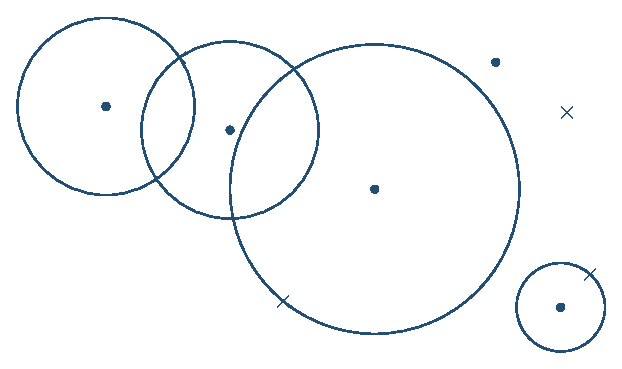
\includegraphics[width=.68\textwidth]{lecture1-fig-01.pdf}
  \FigureTag{L1.1}{fig:lecture1-fig-01}
\end{figure}
Let $(\bullet)$ denote zeros and $(\times)$ poles. If you know
$f^{(n)}(\bullet)$, then you know
\[
  f(z)=\sum_{n\geq0}^{\infty}\frac{f^{(n)}(\bullet)}{n!}(z-\bullet)^n
\]
on a disc that extends up to the nearest pole to $(\bullet)$. Furthermore,
if $f(z)=p(z)/q(z)$, then $(\bullet)$ and $(\times)$ completely determine $f$.
Yet the philosophy says that telling you precisely what $f$ is is not enough
to study its dynamics.
% Author check: the assertion of complete determination by zeros and poles is
% retained verbatim in substance; the source does not mention a multiplicative constant.

Now, here is why this should not surprise you. Let
$\varphi\colon S\to S'$ be a biholomorphism.
\begin{figure}[H]
  \centering
  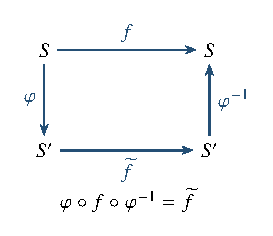
\includegraphics[width=.32\textwidth]{lecture1-fig-02.pdf}
  \FigureTag{L1.2}{fig:lecture1-fig-02}
\end{figure}

% Source page 4
Notice that, since we have merely changed our coordinates (of the surface)
via $f$, the dynamics should remain the same. Indeed, we have:
% Author check: "via f" is the handwritten wording, although the coordinate
% change introduced just above is varphi.
\begin{itemize}
  \item $\widetilde f^{\circ n}=(\varphi\circ f\circ\varphi^{-1})^{\circ n}
  =\varphi\circ f^{\circ n}\circ\varphi^{-1}=\widetilde{f^{\circ n}}$.
  \item If $\{f^{\circ n}|_U\}_n$ is normal, then
  $\{\widetilde f^{\circ n}|_{\varphi(U)}\}_n$ shall be normal.
\end{itemize}
Thus, to study dynamics one must naturally look for things that are invariant
under coordinate transformations. Zeros and poles are not among such
invariants, as can easily be seen. If $f(z_0)=0$, then
$\widetilde f(\varphi(z_0))=\varphi(0)$, which need not be $0$.
But if $\widehat z$ is a fixed or critical point, then:
\begin{itemize}
  \item $\widetilde f(\varphi(z_k))=\varphi(z_k)$, so $\varphi(z_k)$ is a fixed
  point of $\widetilde f$;
  \item $\widetilde f'(\varphi(z_k))=0$, by the chain rule.
\end{itemize}
% Author check: the manuscript changes from z-hat to z_k in these two bullets.
This is the reason for focusing one's study on critical points and fixed
points. Zeros and poles of $f\colon\widehat{\mathbb C}\to\widehat{\mathbb C}$
are merely points that map to the two poles. If you change your coordinates
on $\widehat{\mathbb C}$ via a M\"obius transformation
\[
  z\longmapsto\frac{az+b}{cz+d},
  \qquad \begin{pmatrix}a&b\\c&d\end{pmatrix}\in\operatorname{PSL}_2(\mathbb C),
\]
then the zeros and poles shall be thrown out to points $a/c$, $b/d$ on the
Riemann sphere.
\begin{figure}[H]
  \centering
  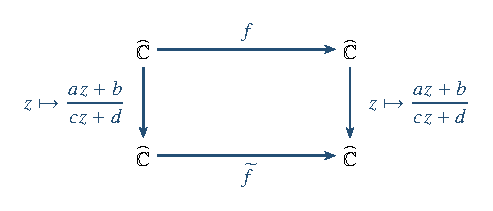
\includegraphics[width=.48\textwidth]{lecture1-fig-03.pdf}
  \FigureTag{L1.3}{fig:lecture1-fig-03}
\end{figure}
Therefore, saying that one wants to study zeros
% Source page 5
and poles of $f$ is equivalent to saying that one has a preferred set of
coordinates. This, mind you, is extremely useful while doing analysis, but
irrelevant for dynamics. One of the many ways we propose to study dynamics is
by reducing the function to a simpler one, in the right set of coordinates.
In particular, if $U\subset S$ and there is
$\varphi\colon U\to\varphi(U)\subseteq\mathbb C$, then among all such
$\varphi$'s we shall hunt for one that makes
$\varphi\circ f\circ\varphi^{-1}$ simplest to study. For instance:
\begin{figure}[H]
  \centering
  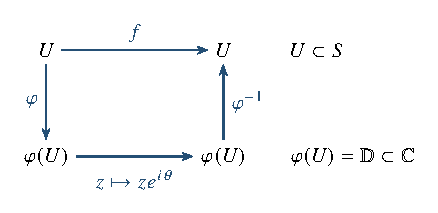
\includegraphics[width=.49\textwidth]{lecture1-fig-04.pdf}
  \FigureTag{L1.4}{fig:lecture1-fig-04}
\end{figure}
Then we know that, under this changed set of coordinates, $f$ is an irrational
rotation by the angle $\theta$ on $\mathbb D$.
\begin{figure}[H]
  \centering
  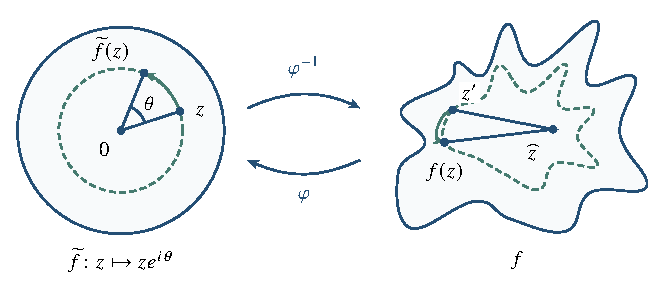
\includegraphics[width=.84\textwidth]{lecture1-fig-05.pdf}
  \FigureTag{L1.5}{fig:lecture1-fig-05}
\end{figure}

% Source page 6
Such results are called \emph{linearization theorems}: one turns the function
into as linear a function as possible, and the orbits of critical points bound
the largest possible domain $U$ in which $f$ behaves like a polynomial.
Usually these domains are considered to be neighbourhoods of fixed points of
$f$. In addition, orbits of critical points reveal a lot of the topological
structure of Julia sets (or chaotic sets). Therefore, the following question
is fundamental to complex dynamics.

\paragraph{Question.}
How is $\{f^{\circ n}(\widehat z)\}_n$ distributed on $S$, where $\widehat z$
is a critical point of $f$?

Ergodic theory comes along with many qualitative answers to such questions.
In this course we shall focus only on those that shall lead us to the proof
of Szemer\'edi's theorem. Having motivated the need for ergodic theory for me,
I encourage you to find a need of your own that would help you cling on to
the kind of mathematics we shall be doing.

\subsection{Introduction to Measure-Preserving Systems}
Let $X$ be a set and $T\colon X\to X$ a map. We shall refer to $X$ as the
\emph{state space} and $T$ as the \emph{transformation} (or deformation).

% Source page 7
If, in addition, you impose some structure on $X$, then we end up with the
following.
\begin{description}[style=nextline,leftmargin=1.5em,labelindent=0pt]
  \item[Group structure.]
  If $\Gamma\triangleleft G$, or $\Gamma<G$, then there is a transitive
  $G$-action on $G/\Gamma$, a homogeneous space of $G$. If $X\cong G/\Gamma$,
  then one has the transformation $T_g\colon X\to X$, $T_g(x):=g\cdot x$.
  One can study the dynamics of $T_g$: a classical dynamical system.
  \item[Topological structure.]
  We study the dynamics of $T\colon X\to X$, with $T$ a continuous map. If,
  in addition, $X$ is compact and metrizable and $T$ is a homeomorphism, one
  is in the realm of topological dynamical systems.
  \item[Measure structure.]
  If it is a probability measure, one ends up with ergodic theory.
\end{description}
Of the three basic structures one can impose on a set, we shall impose the
structure of a probability space. I will end by introducing the setup of
ergodic theory.

% Source page 8
\setcounter{definition}{2}\begin{definition}[Measure-preserving system]
Let $(X,\mathcal B,\mu)$ and $(Y,\mathcal C,\nu)$ be probability spaces. A
measurable map $\varphi\colon X\to Y$ is \emph{measure-preserving} if
\[
  \mu\bigl(\varphi^{-1}(B)\bigr)=\nu(B)
  \qquad\text{for every }B\in\mathcal C,
\]
and $\mu$ is said to be \emph{$\varphi$-invariant}. Finally,
$(X,\mathcal B,\mu,T)$ is a \emph{measure-preserving system} if $\mu$ is
$T$-invariant.
\end{definition}
% Author check: the source uses "varphi-invariant" for the map between two
% possibly different probability spaces, not just for a self-map.

\begin{remark}
\leavevmode\par
\begin{itemize}
  \item To obtain qualitative results, we need some means to compare, so we
  introduce a measure-theoretic structure on our state space $X$. We shall
  address the need for it to be a probability measure later.
  \item Probabilistically, $\varphi\colon X\to Y$ being measurable means that
  events of $Y$ relate to events of $X$.
  \item $\mu$ being $\varphi$-invariant means that the link $\varphi^{-1}$ is
  deterministic. In other words, the likelihood of the occurrence of $B$
  forces the likelihood of the occurrence of $\varphi^{-1}(B)$ to the same
  extent.
  \item $(X,\mathcal B,\mu,T)$ is a space of events with a deterministic link
  function $T$.

% Source page 9
  \item The reason we define $\mu(T^{-1}(B))=\nu(B)$, and not
  $\mu(B)=\nu(T(B))$, is that the following properties do not hold for $T$
  in place of $T^{-1}$:
  \begin{align*}
    \chi_A(T(x))&=\chi_{T^{-1}(A)}(x), &&\text{the link},\\
    T^{-1}(A\cap B)&=T^{-1}(A)\cap T^{-1}(B),\\
    T^{-1}(A\cup B)&=T^{-1}(A)\cup T^{-1}(B),\\
    T^{-1}(A\mathbin\triangle B)&=T^{-1}(A)\mathbin\triangle T^{-1}(B).
  \end{align*}
  If $A$ and $B$ occur, then $T^{-1}$ forces $T^{-1}(A)$ and $T^{-1}(B)$ to
  occur. $T$ does not respect set-theoretic operations, so working with $T$
  would imply that the measure-preserving map is too special!
\end{itemize}
\end{remark}

Having seen this, let us see what it means to preserve the structure of a
measure-preserving system on $X$.
\setcounter{definition}{3}\begin{definition}[Measurable isomorphism]
We write
\[
  (X,\mathcal B_X,\mu_X,T)\cong(Y,\mathcal B_Y,\mu_Y,S)
\]
if there exists a measure-preserving map $\varphi\colon X\to Y$ with
$\varphi^{-1}\colon Y\to X$, where $\varphi$ and $\varphi^{-1}$ are defined
almost everywhere, such that the following diagram commutes.
\end{definition}
\begin{figure}[H]
  \centering
  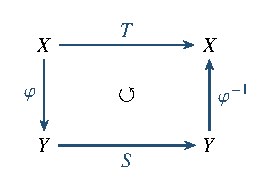
\includegraphics[width=.30\textwidth]{lecture1-fig-06.pdf}
  \FigureTag{L1.6}{fig:lecture1-fig-06}
\end{figure}

% Source page 10
At this point one must ask: how does one check for the measure-preserving
property? Is there a litmus test?

\setcounter{theorem}{0}\begin{lemma}[Litmus test]
Given $(X,\mathcal B,\mu,T)$, with $T\colon X\to X$ measurable, $T$ will be
$\mu$-invariant if $T$ preserves measures of the semi-algebra that generates
$X$.
\end{lemma}
% Author check: "T will be mu-invariant" and "generates X" are the source's
% terminology; no mathematical repair has been made.
\begin{proof}
Let
\[
  \mathcal J'=\{B\in\mathcal B:T^{-1}(B)\in\mathcal B,
  \ \mu(T^{-1}(B))=\mu(B)\}.
\]
Then the semi-algebra $\mathcal J\subseteq\mathcal J'$. The algebra generated
by $\mathcal J$ lies in $\mathcal J'$. Moreover, $\mathcal J'$ is a monotone
class, because if $A_i\nearrow A$, then $T^{-1}(A_i)\nearrow T^{-1}(A)$;
as $\mu(T^{-1}(A_i))=\mu(A_i)$, we have
\[
  \lim_{i\to\infty}\mu(T^{-1}(A_i))=\mu(T^{-1}(A))=\mu(A).
\]
Similarly, one deals with $A_i\searrow A$. Thus $\mathcal J'$ is a
$\sigma$-algebra containing $\mathcal J$, but $\mathcal B$ is, by definition,
the smallest such set of sets. Hence $\mathcal J'=\mathcal B$, so $T$ is
$\mu$-invariant.
\end{proof}

A good time to stop, breathe, and look at examples.
\setcounter{example}{0}\begin{example}[Measure-preserving systems]
\leavevmode\par
\begin{enumerate}
  \setcounter{enumi}{0}\item \emph{Rotation:}
  $(\mathbb R/\mathbb Z,m_{S^1},\mathcal B_{S^1},R_\alpha)$, where
  $R_\alpha\colon\mathbb R/\mathbb Z\to\mathbb R/\mathbb Z$ and
  $R_\alpha(t)=t+\alpha\pmod1$.
  \setcounter{enumi}{1}\item \emph{Doubling:}
  $(\mathbb R/\mathbb Z,m_{S^1},\mathcal B_{S^1},T_2)$, where
  $T_2\colon\mathbb R/\mathbb Z\to\mathbb R/\mathbb Z$ and
  $T_2(t)=2t\pmod1$.
  \setcounter{enumi}{2}\item \emph{Bernoulli shift:}
  $\bigl(\{0,1\}^{\mathbb N},\prod_{\mathbb N}\mu_{1/2},\mathcal B,\sigma\bigr)$,
  where $\mu_{1/2}(\{0\})=\mu_{1/2}(\{1\})=1/2$, and
  $\mu=\prod_{\mathbb N}\mu_{1/2}$ is the product measure, with
  $\sigma(x_0,x_1,x_2,\ldots)=(x_1,x_2,\ldots)$.
\end{enumerate}
\end{example}
% Author check: the order (space, measure, sigma-algebra, transformation) in
% these examples is retained from the manuscript.

% Source page 11
\setcounter{example}{1}\begin{example}[Measurable isomorphism]
Define $\phi\colon\{0,1\}^{\mathbb N}\to\mathbb R/\mathbb Z$ by
\[
  \phi((x_0,x_1,\ldots)):=\sum_{n=0}^{\infty}\frac{x_n}{2^{n+1}}.
\]
$\phi^{-1}$ is not well-defined on rationals in base $2$ (the dyadic
rationals, $\mathbb Z[1/2]$), because they do not have a unique base-$2$
representation. $\mathbb Z[1/2]$ is countable in $\mathbb R/\mathbb Z$, hence
has Lebesgue measure $0$, so $\phi^{-1}$ is invertible.
% Author check: the final assertion is "phi^{-1} is invertible" in the source.
To prove $\mu(\phi^{-1}((a,b)))=m_{S^1}((a,b))=b-a$, it is enough to prove
it for $a=0$ and $b\in\mathbb Q\cap[0,1)$, because, given any
$(a,b)\subseteq[0,1)$,
\begin{align*}
  \mu(\phi^{-1}((a,b)))
  &=\mu\bigl(\phi^{-1}((b,0)\setminus(a,0))\bigr)\\
  &=\mu\bigl(\phi^{-1}((b,0))\setminus\phi^{-1}((a,0))\bigr)\\
  &=\mu(\phi^{-1}((b,0)))-\mu(\phi^{-1}((a,0))).
\end{align*}
% Author check: intervals (b,0) and (a,0), rather than (0,b) and (0,a), are
% written repeatedly in the original and retained here.
Also, given any $(a,b)\subseteq[0,1]$, there exist
$p_n,q_n\in\mathbb Q\cap[0,1)$ such that $(p_n,q_n)\nearrow(a,b)$.

Now note that
\[
  \mu(\phi^{-1}((0,a)))=\mu\left(\bigcup_{i=1}^{n}A_i\right),
\]
where, if $a=0.10010011$,
\[
  A_1=\{0\}\times\{0,1\}^{\mathbb N},\qquad
  A_2=\{1,0,0,0\}\times\{0,1\}^{\mathbb N},\qquad\ldots,
\]
and $A_i=\{1,0,0,1,0,0,\ldots,\underset{i}{0}\}\times\{0,1\}^{\mathbb N}$,
where $i$ is the position of the next $1$ in the base-$2$ expansion of $a$.
Thus
\[
  \mu\left(\bigcup A_i\right)=\sum\mu(A_i)
  =\sum_{\substack{1\text{ in the}\\i\text{th place}}}\frac1{2^i}=a=a-0.
\]
% Author check: finite upper index n, braces for binary prefixes, and the
% indexing of A_i are retained as written; the cylinder notation is informal.
Also, $\phi\circ\sigma=T_2\circ\phi$. Hence the Bernoulli system is
measurably isomorphic to the circle-doubling system.
\end{example}

\subsection{Our Goals and Motives}
We have a means to measure, hence a way to compare, and we wish to compare
$E$ with its iterates $T^{\circ n}(E)$. As $T$ is measure-preserving, we are
justified in asking how $\{T^{\circ n}(E)\}_n$ behaves, because $T$ preserves
measure, so $E$ and $T(E)$ belong to the same structural space; hence
comparison is natural.

% Source page 12
\Needspace{9\baselineskip}
With that in mind, we ask the following questions:
\begin{itemize}
  \item What happens to $\{T^{\circ n}x\}$ as $n\to\infty$?
  \item What happens to $T^{\circ n}(E)$ as $n\to\infty$, for $E\in\mathcal B$?
  \item What happens to $f\circ T^n$ as $n\to\infty$, for measurable
  $f\colon X\to\mathbb R$ (or $\mathbb C$)?
\end{itemize}
We shall develop tools and techniques to understand the implications of these
questions, and answer them to the extent we can, culminating in Furstenberg's
multiple recurrence theorem (FMRT).

\setcounter{theorem}{1}\begin{theorem}[Furstenberg's multiple recurrence theorem (FMRT)]
Let $(X,\mathcal B,\mu,T)$ be a measure-preserving system. Let
$E\in\mathcal B$ satisfy $\mu(E)>0$, and let $k\geq1$. Then there exists
$n\geq1$ such that
\[
  E\cap T^n(E)\cap\cdots\cap T^{(k-1)n}(E)\neq\varnothing.
\]
Equivalently, there exist $x\in X$ and $n\geq1$ such that $T^{\ell n}(x)\in E$
for every $0\leq\ell<k$.
\end{theorem}
% Author check: the source uses positive powers on the sets, and gives the
% displayed orbit statement as equivalent; no alteration has been made.
From this we get a combinatorial analogue:
\setcounter{theorem}{2}\begin{theorem}[Szemer\'edi's theorem]
Let $E\subset\mathbb Z$ satisfy
\[
  \limsup_{N\to\infty}\frac{|E\cap[-N,N]|}{2N+1}>0.
\]
Then $E$ has arbitrarily large arithmetic progressions.
\end{theorem}
And declare victory!
% BLOG-CONTENT-END
\end{document}
